\documentclass[a4paper]{article}
\usepackage{amsfonts}
\usepackage{a4wide,times}
\usepackage[english]{babel}
\usepackage{graphicx}
\usepackage{listings}
\usepackage[parfill]{parskip}
\lstset{language=Java,
  numberstyle=\footnotesize,
  basicstyle=\footnotesize,
  numbers= left,
  stepnumber=1,
  tabsize=2,
  frame=shadowbox,
  breaklines=true
}


\begin{document}

\title{Net-computing\\
Architectural design document\\
Smart car on demand
}

\date{\today}

\author{Peri Rahamin (s2683423),\\
Jits Schilperoort (s2788659),\\
Twan Schoonen (s2756978)
}




\maketitle
\section*{Project description}
Smart car on demand is the name of our project idea to have self-driving cars drive through the city, and get ordered by customers who wish to go somewhere using this service. The order is done by a costumer logging in to a mobile application, and select their destination and number of passengers.

The request has the user's location saved, is sent to the car center, that selects the nearest car that can handle the request. Payment is done via money that is saved in the app account (top up is required beforehand). Requests are handled in queue order (first order-first served, maybe we add some priority).

The car arrives to the costumer(s) and takes them to their destination. Selecting a car and planning routes are handled by Artificial Intelligence systems that is able to compute the shortest route. The AI also allows the automated cars to drive without human intervention.

Since this is a big project, we will not implement all of the features, but only those relevant for this course. This list specifies the different elements of the system, with an explanation of why we decided to implement or not implement it:
\begin{itemize}
    \item \textbf{Mobile application:} Each costumer that is interested in getting a car to drive them uses a mobile app to make the order. A working app with an user friendly GUI is irrelevant for this course, so we decided to have some data structure that represents a user and has location and number of people who want to use the service instead.
    \item \textbf{AI:} The automated driving cars should know how to drive on roads without the help of humans. The AI of the car should follow the law and consider other cars (agents) or people crossing the road in its surrounding. This part is obviously too much to implement, and since it is also irrelevant to this course, we decided to assume the AI works.
    \item \textbf{Shortest distance algorithm:} We want the car to find the best route to reach its costumer, considering traffic and other parameters (such as construction that blocks the road). The algorithm helps deciding which car is most suitable to get to a costumer, in case there are few of them in different parts of the city. To make this work we need live data, so for this project, we only send messages with datasets we made ourselves, and leave out the complicated calculations.
\end{itemize}
%TODO: add more items to list

\section*{Project requirements}
%TODO: improve list
The requirements that are implemented in this project are listed as follows:
\begin{itemize}
    \item \textbf{Socket:} used for center to car communication, also used for center to center communication. This is done when a destination is in an other center area then to location (longer drives).
    \item \textbf{Message queuing:} the requests made by the mobile application are queued by the centers, the when there are available cars the center dequeus the order and communicates with the car. 
    \item \textbf{Web services (REST):} the mobile app communicates with the database by using REST. This is used for getting client information.
\end{itemize}

\subsection*{Star vs P2P topology}
\textbf{Star topology:} The star topology is used by the centers to control the cars. Here the cars only drive and all computing is done by the center.\\
\textbf{P2P topology:} This method is used for center to center communication, so when a car leaves the district or city, the centers communicate to each other and swap cars.

%TODO: more elaborated description of what information the cars share
\section*{Component diagram}
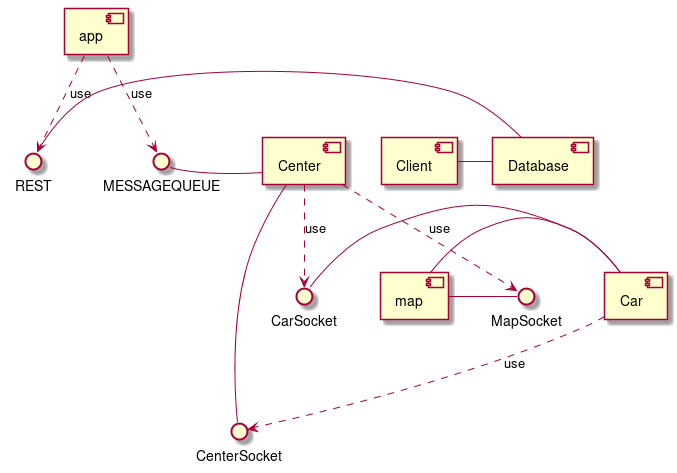
\includegraphics[width=1\textwidth]{../Diagrams/componentDiagram.png}

\section*{Class diagram}
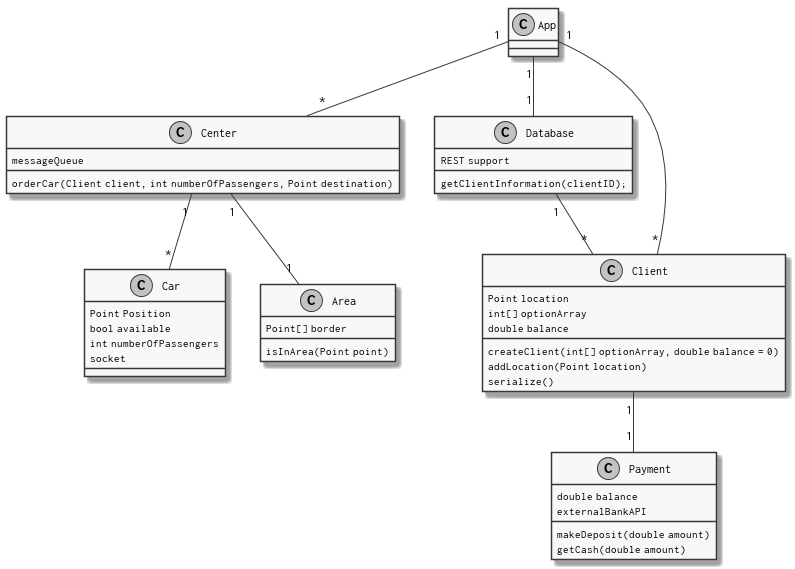
\includegraphics[width=1\textwidth]{../Diagrams/classDiagram.png}

\section*{Sequence diagrams}
\subsection*{OrderCar}
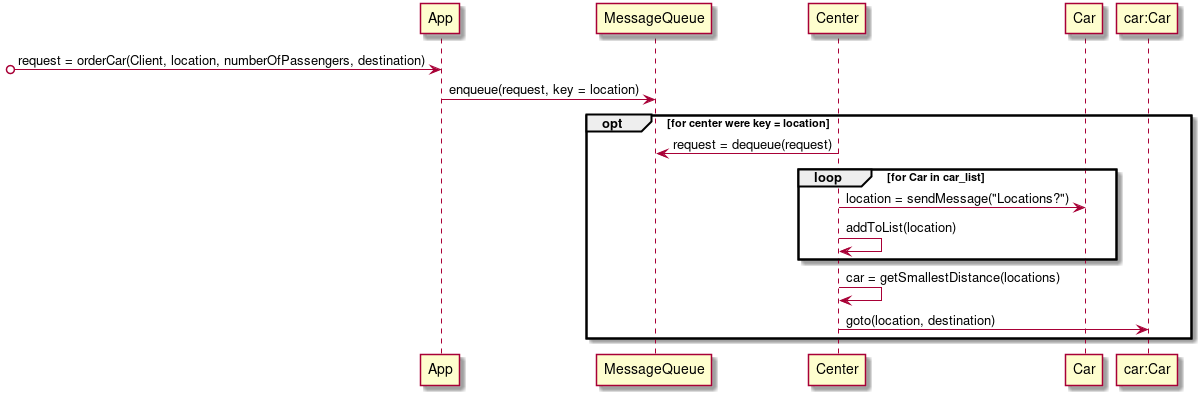
\includegraphics[width=1\textwidth]{../Diagrams/orderCar.png}\\
\subsection*{SendCar}
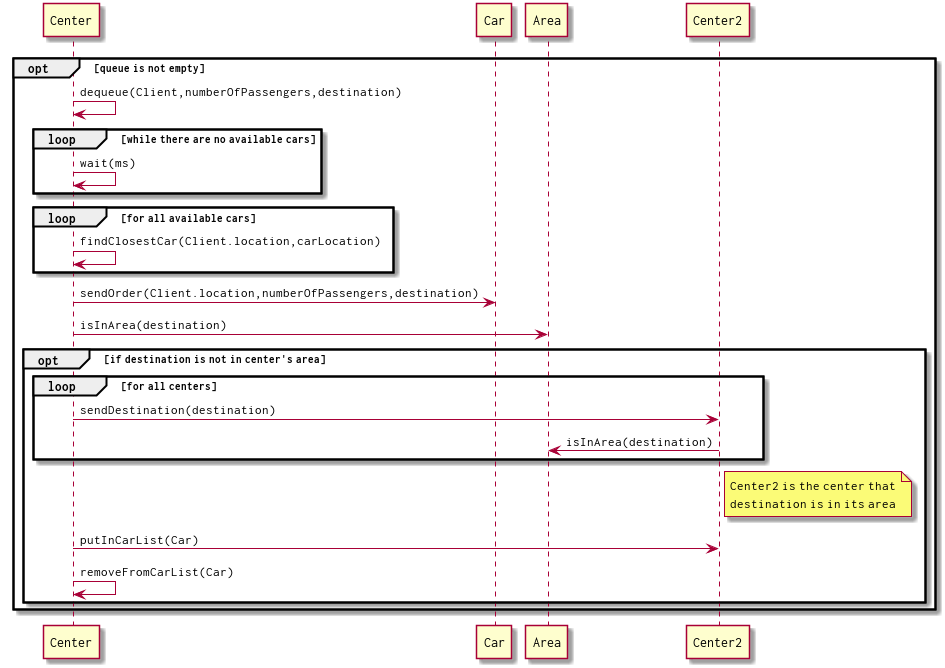
\includegraphics[width=1\textwidth]{../Diagrams/sendCar.png}\\
\subsection*{RegisterClient}
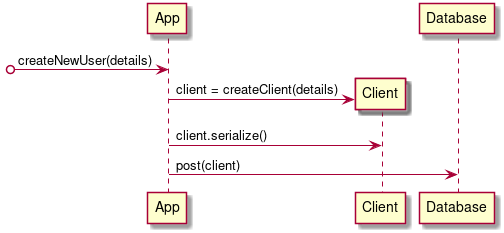
\includegraphics[width=1\textwidth]{../Diagrams/registerClient.png}

\end{document}

